\documentclass[a4paper,11pt]{article}
\usepackage{graphicx}
\usepackage{float}
\usepackage{subfig}
\usepackage{geometry}
\usepackage{amsmath,amssymb}
\usepackage{amsthm}
\usepackage{bbold}
\usepackage{mathtools}
\usepackage{braket}
\usepackage{booktabs}
\usepackage[table,xcdraw]{xcolor}
\usepackage[utf8]{inputenc}
\usepackage{cite}
\usepackage[english]{babel}
\usepackage{lipsum}
\usepackage{setspace}
\usepackage{minted}
\usepackage{xcolor}
\newcommand{\R}{\mathbb{R}}
\usepackage{hyperref}
\hypersetup{colorlinks=true,linkcolor=blue}
\geometry{a4paper, top=2.5cm, bottom=2.5cm, left=3cm, right=2.5cm}

\begin{document}
	\author{Catalano Giuseppe, Cerrato Nunzia}
	\title{Numerical Linear Algebra Homework Project 3:\\Eigenvalues and Eigenvectors}
	\date{}
	\maketitle
	
\section*{Problem 1}
\textbf{(1)}
We want to reduce the symmetric matrix $A$
\begin{equation}\label{key}
	A = \begin{bmatrix}
		4 & -1 & -1 & 0 \\
		-1 & 4 & 0 & -1 \\
		-1 & 0 & 4 & -1 \\
		0 & -1 & -1 & 4
	\end{bmatrix} 
\end{equation}
to a tridiagonal form using Housholder similarity transformations. The matrix $A$ can be expressed in the following, compact way:
\begin{equation}
	A =  \left[ 
\begin{array}{c|ccc}
	a_{11}&  & \textbf{x}^T  &  \\
	\hline
	&  &  &  \\
	\textbf{x}&  & \hat{A}_1 &  \\
	&  &  & 
\end{array}\right] .
\end{equation}
Let us define the vector $\textbf{u}_{1}$
\begin{equation}\label{key}
	\textbf{u}_1 = \textbf{x} + \text{sgn}(x_1) \lVert \textbf{x}\rVert_2 \textbf{e}_1
\end{equation}	
% = \begin{bmatrix}
%		-1-\sqrt{2}\\
%		-1\\
%		0
%	\end{bmatrix},
%\end{equation}
thanks to which we can define the matrix $\hat{R}_1$
\begin{equation}\label{key}
	\hat{R}_1 = \mathbb{1}_3 - \frac{2}{\lVert \textbf{u}_1\rVert_2^2} \textbf{u}_1 \textbf{u}_1^T
\end{equation}
and a new matrix $R_1$, as follows:
\begin{equation}\label{key}
	R_1 = \left[ 
	\begin{array}{c|ccc}
		1 &  & \textbf{0}^T  &  \\
		\hline
		&  &  &  \\
		\textbf{0}&  & \hat{R}_1 &  \\
		&  &  & 
	\end{array}\right] .
\end{equation}
We will not explicitely construct the matrix $R_1$, as we know that the product $R_1 A$ will assume the following form:
\begin{equation}\label{key}
	R_1 A= \left[ 
	\begin{array}{c|ccc}
		a_{11} &  & \textbf{x}^T  &  \\
		\hline
		-\text{sgn}(x_1) \lVert \textbf{x}\rVert_2  &  &  &  \\
		0 &  & \hat{R}_1 \hat{A}_1 &  \\
		0 &  &  & 
	\end{array}\right] ,
\end{equation}
where the first column is obtained by constuction and the matrix $\hat{R}_1\hat{A}_1$ can be obtained by considering the matrix $\hat{A}_1$ written by columns as $\hat{A}_1 = \left[ ( \hat{A}_1)_1,( \hat{A}_1)_2,( \hat{A}_1)_3 \right] $. Hence $\hat{R}_1\hat{A}_1 = \left[ ( \hat{R}_1\hat{A}_1)_1,( \hat{R}_1\hat{A}_1)_2,(\hat{R}_1 \hat{A}_1)_3 \right] $, where we know that a singole column can be computed as:
\begin{equation}\label{key}
	( \hat{R}_1\hat{A}_1)_i = (\hat{A}_1)_i - \frac{2}{\lVert \textbf{u}_1\rVert_2^2} \textbf{u}_1 \textbf{u}_1^T(\hat{A}_1)_i .
\end{equation}
By expliciting all the terms, we obatin:
\begin{equation}\label{key}
	R_1 A = \begin{bmatrix}
		4 & -1 & -1 & 0 \\
		\sqrt{2} & -2\sqrt{2} & -2\sqrt{2} & \sqrt{2} \\
		0 & -2\sqrt{2} & 2\sqrt{2} & 0 \\
		0 & -1 & -1 & 4
	\end{bmatrix}.
\end{equation}
Since we want to obtain a tridiagonal matrix, we have to compute the matrix $R_1 A R_1$, namely:
\begin{equation}\label{key}
	R_1 A R_1 = \left[ 
	\begin{array}{c|ccc}
		a_{11} &  \lVert \textbf{x}\rVert_2 &  0 & 0 \\
		\hline
		 \lVert \textbf{x}\rVert_2  &  &  &  \\
		0 &  & \hat{R}_1 \hat{A}_1 \hat{R}_1  &  \\
		0 &  &  & 
	\end{array}\right].
\end{equation}
 Knowing that $\hat{R}_1 \hat{A}_1 \hat{R}_1 = (\hat{R}_1 \hat{A}_1 \hat{R}_1)^T = (\hat{R}_1)^T (\hat{R}_1 \hat{A}_1 )^T =\hat{R}_1 (\hat{R}_1 \hat{A}_1 )^T$, we can apply $\hat{R}_1$ to $(\hat{R}_1 \hat{A}_1 )^T$ by columns:
 \begin{equation}\label{key}
	\left[ \hat{R}_1 \hat{A}_1 \hat{R}_1 \right]_i = 	\left[ (\hat{R}_1 \hat{A}_1 )^T \right]_i  - \frac{2}{\lVert \textbf{u}_1\rVert_2^2} \textbf{u}_1 \textbf{u}_1^T	\left[ (\hat{R}_1 \hat{A}_1 )^T \right]_i ,
\end{equation}
obtaining the following form for the matrix $R_1 A R_1 $:
\begin{equation}\label{key}
		R_1 A R_1 = \left[ \begin{array}{cccc}
		4 & \sqrt{2} & 0 & 0 \\
		\sqrt{2} & 4 & 0 & \sqrt{2} \\
		0 & 0 & 4 & 0 \\
		0 & \sqrt{2} & 0 & 4
	\end{array} \right] .
\end{equation}
By identifying the submatrix $	\hat{R}_1 \hat{A}_1 \hat{R}_1$ as
\begin{equation}\label{key}
	\hat{R}_1 \hat{A}_1 \hat{R}_1 = \left[ \begin{array}{ccc}
		4 & 0 & \sqrt{2} \\
		0 & 4 & 0 \\
		\sqrt{2} & 0 & 4
	\end{array} \right]  =  \left[ \begin{array}{cc}
	(\hat{R}_1 \hat{A}_1 \hat{R}_1)_{11}& \textbf{y}^T \\
	\textbf{y} & \hat{A}_2 
\end{array} \right],
\end{equation}	
we can build the vector $\textbf{u}_2 $ as
\begin{equation}\label{key}
	\textbf{u}_2 = \textbf{y} + \text{sgn}(y_1) \lVert \textbf{y}\rVert_2\textbf{e}_1^{(2)},
\end{equation}	
%\begin{equation}\label{key}
%	 = \sqrt{2} \begin{bmatrix}
%		1\\
%		1
%	\end{bmatrix}
%\end{equation}	
which will allow us to define the matrix $\hat{R}_2$
\begin{equation}\label{key}
	\hat{R}_2 = \mathbb{1}_2 - \frac{2}{\lVert \textbf{u}_2\rVert_2^2} \textbf{u}_2 \textbf{u}_2^T.
\end{equation}
Using the same logic, we obtain the i-th column of the matrix $\hat{R}_2\hat{A}_2$, namely:
\begin{equation}\label{key}
	( \hat{R}_2\hat{A}_2)_i = (\hat{A}_2)_i - \frac{2}{\lVert \textbf{u}_2\rVert_2^2} \textbf{u}_2 \textbf{u}_2^T(\hat{A}_2)_i,
\end{equation}
and, by expliciting all the terms we obtain:
\begin{equation}\label{key}
	\hat{R}_2 \hat{A}_2 = \left[ \begin{array}{cc}
		0 & -4 \\
		-4 & 0
	\end{array}\right].
\end{equation}
As before, we can compute $\hat{R}_2 \hat{A}_2 \hat{R}_2$ by columns, and the final form of the matrix will be:
\begin{equation}\label{key}
	R_2R_1AR_1R_2 =\begin{bmatrix}
		4& \sqrt{2} & 0  &  0\\
		\sqrt{2}&4 & -\sqrt{2} & 0\\
		0 & -\sqrt{2} & 4  & 0 \\
		0 & 0 & 0 & 4
	\end{bmatrix}.
\end{equation}
As we can see, we have reduced the initial matrix $A$ to tridiagonal form.\\

\noindent \textbf{(2)} In the following we report the script where we implement the QR diagonalization of a matrix $A$, defined as:
\begin{equation}
	A = \begin{bmatrix}
		4 & 3 & 2 & 1 \\
		3 & 4 & 3 & 2 \\
		2 & 3 & 4 & 3 \\
		1 & 2 & 3 & 4
	\end{bmatrix}.
\end{equation}

\begin{minted}[mathescape, linenos, breaklines]{python}
import numpy as np
import matplotlib.pyplot as plt

# Set the initial values
tol = 1e-5
counter = 0
t = 1 # Initial exponent for the tolerance

# Set the number of significant digits
np.set_printoptions(precision=15, suppress=True)

# Construct the matrix A
A = np.array([[4,3,2,1],[3,4,3,2],[2,3,4,3],[1,2,3,4]])
# Compute the exact eigenvalues
exact_eigenvalues = np.linalg.eigvals(A)

# Initialize an empty list to store the number of iterations at each t
t_counter_list = []

# Cycle until the stopping criterion is not satisfied
while np.amax(np.abs(A - np.diag(np.diag(A)))) >= tol:
 # Obtain the QR factorization of A and perform the QR iteration
 Q, R = np.linalg.qr(A)
 A = R@Q

 # Obtain the current approximation of the eigenvalues
 computed_eigvals = np.diag(A)

 # Compute and store the maximum absolute error on the eigenvalues
 abs_error = max(np.abs(exact_eigenvalues - computed_eigvals))

 counter += 1

 if abs_error < 10**(-t):
   t_counter_list.append(counter)
   t += 1

 if counter in [1,5,10,15]:
   print(f'k={counter}')
   print(A)
   print('--------------------------')
print(f'Final k = {counter}')
print(A)
computed_eigvals = np.diag(A)

print('------------------------')
print(f'Exact eigenvalues = {format(exact_eigenvalues)}')
print(f'Computed eigenvalues = {format(computed_eigvals)}')
diff_eigvals = np.abs(exact_eigenvalues - computed_eigvals)
print(f'Absolute error = {format(diff_eigvals)}')
\end{minted}

\noindent Here we report the intermediate $A_k$ matrices for $k = 1, 10, 15, 15$ and the final one with $k = 21$ and the exact and computed eigenvalues, with the absolute errors.

\begin{minted}{text}
k=1
[[ 9.733333333333334  2.834948829502994  0.878364340955178 -0.231869447880085]
[ 2.834948829502991  3.783908045977011  1.539932953851869 -0.60279905751826 ]
[ 0.878364340955178  1.539932953851869  1.515016685205784 -0.509164636937078]
[-0.231869447880084 -0.602799057518259 -0.509164636937078  0.967741935483871]]
--------------------------
k=5
[[11.098895703904493  0.030845371708295  0.000040119600318 -0.000003286456335]
[ 0.030845371708295  3.414318666854397  0.006815571252927 -0.000792986818634]
[ 0.000040119600319  0.006815571252927  0.884533164554776 -0.070136316449804]
[-0.000003286456334 -0.000792986818633 -0.070136316449804  0.602252464686331]]
--------------------------
k=10
[[11.099019512653443  0.000084962498578  0.00000000014034  0.000000000001383]
[ 0.000084962498578  3.414213563282151  0.000008722995681  0.000000121056837]
[ 0.00000000014034   0.000008722995681  0.900746172772326  0.008590655965716]
[ 0.000000000001382  0.000000121056836  0.008590655965716  0.586020751292075]]
--------------------------
k=15
[[11.099019513592774  0.000000234022501  0. -0.000000000000001]
[ 0.000000234022501  3.414213562373102  0.000000011163285 -0.000000000018006]
[ 0.                 0.000000011163285  0.900977321539928 -0.000998767899781]
[-0.                -0.000000000018005 -0.000998767899781  0.585789602494192]]
--------------------------
Final k = 26
[[11.099019513592783  0.000000000000546 -0.  0.000000000000001]
[ 0.000000000000546  3.414213562373094  0.000000000000005  0.000000000000001]
[ 0.                 0.000000000000005  0.900980486163497  0.000008764600757]
[ 0.                 0.                 0.000008764600758  0.585786437870623]]
--------------------------
Exact eigenvalues = 
[11.099019513592786  3.414213562373094  0.900980486407215  0.585786437626905]
Computed eigenvalues =
[11.099019513592783  3.414213562373094  0.900980486163497  0.585786437870623]
Absolute error =
[0.000000000000004 0.                0.000000000243718 0.000000000243717]
\end{minted}

\noindent We can observe the decreasing of the off-diagonal entries and the convergence of the diagonal terms to the eigenvalues computed using the function np.linalg.eigvals, which we consider as exact. The maximum absolute error on the eigenvalues is of the order of $10^{-8}$.\\

\noindent In the following script we implement the QR diagonalization of the matrix $A$ using the Rayleigh quotient shift and deflation. \\

\begin{minted}[mathescape, linenos, breaklines]{python}
# Initialize values
t = 9
tol_list = 10.**(-np.array(range(1,t)))
counter_list = []

# Construct the matrix A
A = np.array([[4,3,2,1],[3,4,3,2],[2,3,4,3],[1,2,3,4]])
# Compute the exact eigenvalues
exact_eigenvalues = np.linalg.eigvals(A)
exact_eigenvalues_copy = exact_eigenvalues.copy()

# Cycle on the list of tolerances
for tol in tol_list:
  counter = 0
  A = np.array([[4,3,2,1],[3,4,3,2],[2,3,4,3],[1,2,3,4]])
  exact_eigenvalues = exact_eigenvalues_copy.copy()
  dim = np.shape(A)[0]

  # Perform QR iteration until the matrix is reduced to a single value by deflation
  while dim > 0:
    approx_lambda = A[dim-1,dim-1]
    eig_error = abs(exact_eigenvalues-approx_lambda)
    # If the error on an eigenvalue is less than the tolerance, perform deflation
    if min(eig_error) < tol:
       index = np.argmin(eig_error)
       exact_eigenvalues = np.delete(exact_eigenvalues,index)
       A = A[:dim-1,:dim-1]
       dim = dim - 1 
       continue

    # Compute the shift and perform QR iteration
    shift = A[dim-1,dim-1]
    Q, R = np.linalg.qr(A - shift * np.eye(dim))
    A = R@Q + shift * np.eye(dim)
    counter = counter + 1

  counter_list.append(counter)
\end{minted}

\begin{figure}[H]
	\centering
	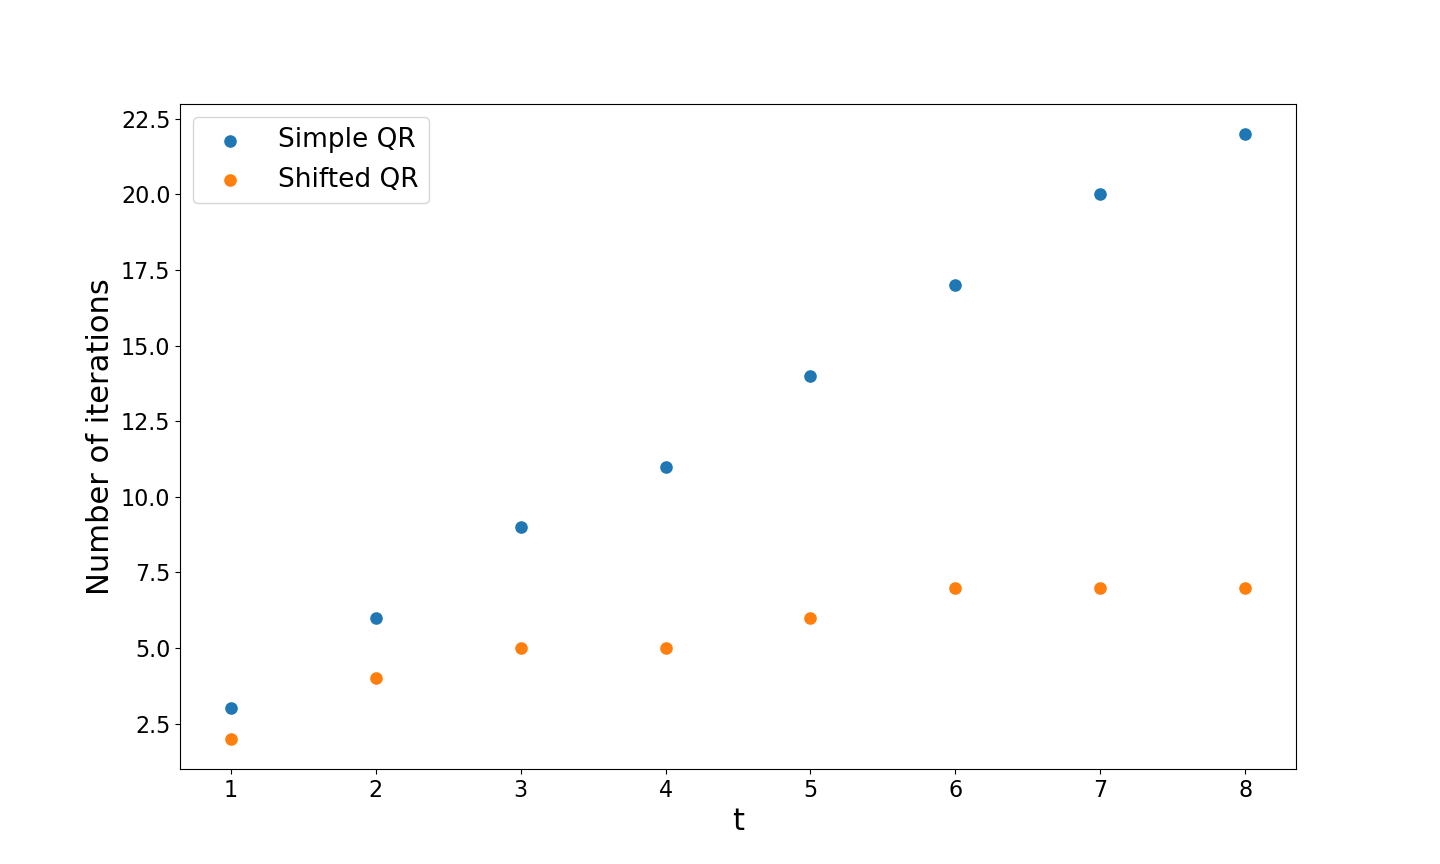
\includegraphics[scale=0.40]{Plot/Plot_QR_Standard_Rayleigh.png}
	\caption{Number of iteration needed to achieve a maximum absolute error less than $10^{-t}$ on the eigenvalues computed by using standard and shifted QR iteration algorithm.}
	\label{Fig:Num_iter_with_t}
\end{figure}

\noindent As we see from Fig. \ref{Fig:Num_iter_with_t}  the number of iteration required to achieve a maximum absolute error less than $10^{-t}$ on eigenvalues appears to grow linearly with $t$ in the case of the simple QR iteration algorithm. On the other hand, in the case of the shifter QR iteration algorithm, implemented by using the Rayleigh shift, the same error appears to grow sublinearly with $t$, meaning that this last algorithm reaches the required tolerance with a less number of iterations, thus being faster.

	
\section*{Problem 2}	
We want to find approximations to the eigenvalues and eigenfunctions of the one-dimensional Laplace operator $L[u] := - \frac{d^2 u }{dx^2}$ on the unit interval $[0,1]$ with boundary conditions $u(0) = u(1) = 0$. Let us define as $\lambda_{i}$ an eigenvalue of $L$ and as $u_{i}$  the corresponding eigenfunction.
%
%A scalar $\lambda$ is said to be an eigenvalue of $L$ (with homogeneous Dirichlet boundary conditions) if there exists a twice-differentiable function $u : [0, 1] \rightarrow \R$, not identically zero in $[0, 1]$, such that
%\begin{equation}\label{eq: continuous differential eigenproblem}
%	-u''(x) = \lambda u(x) \text{ on } [0,1] \text{ with } u(0) = u(1) = 0.
%\end{equation}
%In this case $u$ is said to be an \textit{eigenfunction} of $L$ corresponding to the eigenvalue $\lambda$. Obviously, eigenfunctions are defined up to a nonzero scalar multiple.
%
%The eigenvalues and eigenfunctions of $L$ are easily found to be $\lambda_j = j^2\pi^2$ and $u_j(x) = \alpha \sin(j\pi x)$ for any nonzero constant $\alpha$, which we can take to be $1$. Here $j$ is a positive integer; hence, the operator $L$ has an infinite set of (mutually orthogonal) eigenfunctions $\{u_j\}_{j=1}^\infty $ corresponding to the discrete spectrum of eigenvalues ${\lambda_j}_{j=1}^\infty $. Note that $0 < \lambda_1 < \lambda_2 < \dots < \lambda_j \rightarrow \infty$ as $j \rightarrow \infty$. Also, each eigenvalue is simple in the sense that (up to a scalar multiple) there is a unique eigenfunction corresponding to it.

\noindent Approximations to the eigenvalues and eigenfunctions can be obtained by discretizing the interval $[0, 1]$ by means of $N+2$ evenly spaced points: $x_i =ih \text{ where } i=0,1,...,N+1 \text{ and } h=1/(N+1)$. The second derivative operator can then be approximated by centred finite differences:

\begin{equation}
	-\frac{d^2u}{dx^2}(x_i) \approx \frac{-u(x_{i-1} + 2 u(x_i)  -2 u(x_{i+1}) )}{h^2}
\end{equation}
and therefore the continuous (differential) eigenproblem can be approximated by the discrete (algebraic) eigenvalue problem 

\begin{equation}\label{key}
	h^{-2} T_N \textbf{u} = \lambda \textbf{u},
\end{equation}
where we have set

\begin{equation}\label{key}
	T_N = \begin{bmatrix}
		2 & -1 &  & 0 \\
		-1 & \ddots  & \ddots  &  \\
		& \ddots & \ddots & -1 \\
		0 &  & -1 & 2
	\end{bmatrix}, \text{ and } \textbf{u} = \begin{bmatrix}
		u_1\\
		u_2\\
		\vdots\\
		u_N
	\end{bmatrix},
\end{equation}
with $u_i := u(x_i)$. Recall that the eigenvalues and eigenfunctions of $L$ are $\lambda_j = j^2\pi^2$ and $u_j(x) = \alpha \sin(j\pi x)$ for any nonzero constant $\alpha$, which we can take to be $1$, and $j$ positive integer. On the other hand, the $N \times N$ matrix $T_N$ has eigenvalues $\mu_j = 2(1- \cos \frac{\pi j }{N+1})$ for $j = 1, \dots, N$, corresponding to the eigenvectors $\textbf{u}_j$, where $\textbf{u}_j(k) = \sqrt{\frac{2}{N+1}} \sin\big( \frac{j k \pi}{N+1} \big)$ is the $kth$ entry in $\textbf{u}_j$.

%Notice that the eigenvectors $\textbf{u}_j$ are normalized with respect to the 2-norm: $\textbf{u}^T_j \textbf{u}_j = 1$. Also notice that the eigenvalues of $T_N$ lie in the interval $(0, 4)$. Hence, the eigenvalues of $h^{-2} T_N$ lie in the interval $(0, 4(N + 1)2 )$.\\


\noindent \textbf{(1)} Since we are considering $j\ll N$ and $N\gg1$ we can consider the Taylor expansion of $\cos \left( \frac{\pi j }{N+1}\right) $,
%\begin{equation}
%	\cos \frac{\pi j }{N+1} = \cos \pi j h = 1 - \frac{1}{2!} (\pi j h)^2 + \frac{1}{4!} (\pi j h)^4 + O(h^6),
%\end{equation}
which leads us to approximate the smallest eigenvalues of $2h^{-2} T_N$ as follows:
\begin{equation}\label{Eq:Taylor_exp_small_j}
	2h^{-2} \left( 1- \cos \frac{\pi j }{N+1} \right)  = 2h^{-2} \left(\frac{(\pi j h)^2}{2!} - \frac{(\pi j h)^4}{4!} + O(h^6)\right)  = \pi^2 j^2 \left( 1- \frac{(\pi j h)^2}{12} + O(h^4) \right),
\end{equation}
where we used that $h=1/N+1$.\\
\noindent For the largest eigenvalue of $T_N$, we have that $j = N$, therefore we can not truncate anymore the Taylor expansion of the cosine if we want a good approximation. We can compute the $N-th$ eigenvalue of $T_N$ in the limit of $N\gg 1$ (namely $h\ll 1$):
\begin{equation}\label{Eq:Taylor_exp_big_j}
	\mu_N = 2\left( 1-\cos\pi  \frac{N}{N+1}\right)   =2(1-\cos (\pi -\pi h) ) = 2(1+\cos\pi h) = 4 - \pi^2 h^2 + O(h^4).
\end{equation}
Therefore, we have
\begin{equation}\label{key}
	h^{-2} \mu_N = \frac{4}{h^2} - \pi^2 + O(h^2) =4(N+1)^2 - \pi^2 + O(N^{-2}),
\end{equation}
which is not a good approximation of $\lambda_N = \pi^2 N^2$.

\noindent \textbf{(2)} We want to compare the eigenvectors $\textbf{u}_j$ of $T_N$ with the eigenfunctions of $L$, up to the normalization constant, that we will set to $1$ for both. If we recall that $x_k = k h\ \forall k = 1,\dots, N$, we can observe that the $k-th$ component of the eigenvector $\textbf{u}_j$ is equal to the $j-th$ eigenfunction $u_j(x)$ computed in corrispondence of the value $x=x_k$:
\begin{equation}
	u_j(x_k) = \sin(j \pi x_k) = \sin ( j \pi k h ) = \sin\left( \frac{j \pi k}{N+1}\right)  = \textbf{u}_j(k).
\end{equation}

\noindent \textbf{(3)}  Now we compute the spectral condition number of $T_N$, defined as 	$k_2(T_N) = \frac{h^{-2}\mu_N}{h^{-2}\mu_1}$, in the limit of $N\gg 1$. We recall that the eigenvalues of $T_N$ are
\begin{equation}\label{key}
	\mu_j = 2\left( 1-\cos \frac{\pi j}{N+1}\right) = 2\left( 1-\cos \pi j h\right).
\end{equation}

\noindent By considering the Taylor expansion of the cosine, we can compute the numerator and the denominator of $k_2(T_N)$. In particular, to compute the numerator we can use the expression reported in Eq. \eqref{Eq:Taylor_exp_small_j}, where $j=1$, while for the denominator we use the expression reported in Eq. \eqref{Eq:Taylor_exp_big_j}.
%\begin{equation}
%	\begin{split}
%		h^{-2}\mu_N &= h^{-2}2(1+\cos(\pi h))\\
%		&=2h^{-2} \left( 1 + 1 -\frac{1}{2} \pi^2 h^2 + \frac{1}{4!} \pi^4 h^4 + O(h^6)\right) \\
%		&= 4 h^{-2} - \pi^2 +\frac{1}{12} \pi^4 h^2 + O(h^4)
%	\end{split}
%\end{equation}
%\begin{equation}
%	\begin{split}
%		h^{-2}\mu_1 = h^{-2} 2 \left(  1-1 +\frac{1}{2} \pi^2 h^2 - \frac{1}{4!} \pi^4 h^4 + O(h^6)\right) = \pi^2 -\frac{1}{12} \pi^4 h^2 + O(h^4)
%	\end{split}
%\end{equation}
\begin{equation}
	k_2(T_N) = \frac{h^{-2}\mu_N}{h^{-2}\mu_1} = \frac{4 h^{-2} - \pi^2 +\frac{1}{12} \pi^4 h^2 + O(h^4)}{\pi^2(1 -\frac{1}{12} \pi^2 h^2 + O(h^4))}.
\end{equation}
Here, in the denominator, we can use the expansion $ (1+x)^\alpha = 1+\alpha x + O(x^2) $, finding $ (1 -\frac{1}{12} \pi^2 h^2 + O(h^4))^{-1} = 1 + \frac{1}{12} \pi^2 h^2 + O(h^4) $. Therefore, we find
\begin{equation}\label{key}
\begin{split}
	k_2(T_N) &=\left(  \frac{4 h^{-2}}{\pi^2} - 1 +\frac{1}{12} \pi^4 h^2 + O(h^4)\right) \left( 1 + \frac{1}{12} \pi^2 h^2 + O(h^4) \right)\\
	&= \frac{4 h^{-2}}{\pi^2} - 1 +\frac{1}{12} \pi^4 h^2 + \frac{4 h^{-2}}{\pi^2} \frac{1}{12} \pi^2 h^2 -\frac{1}{12} \pi^2 h^2+ O(h^4) \\
	&= \frac{4 h^{-2}}{\pi^2} - \frac{2}{3} + O(h^2)= \frac{4 (N+1)^2}{\pi^2} - \frac{2}{3} + O(N^{-2}).
\end{split}
\end{equation}

\noindent \textbf{(4-5)} Here we report the plot of the eigenvalues and eigenvectors of $T_{N}$, with $N=21$.

\begin{figure}[H]
	\centering
	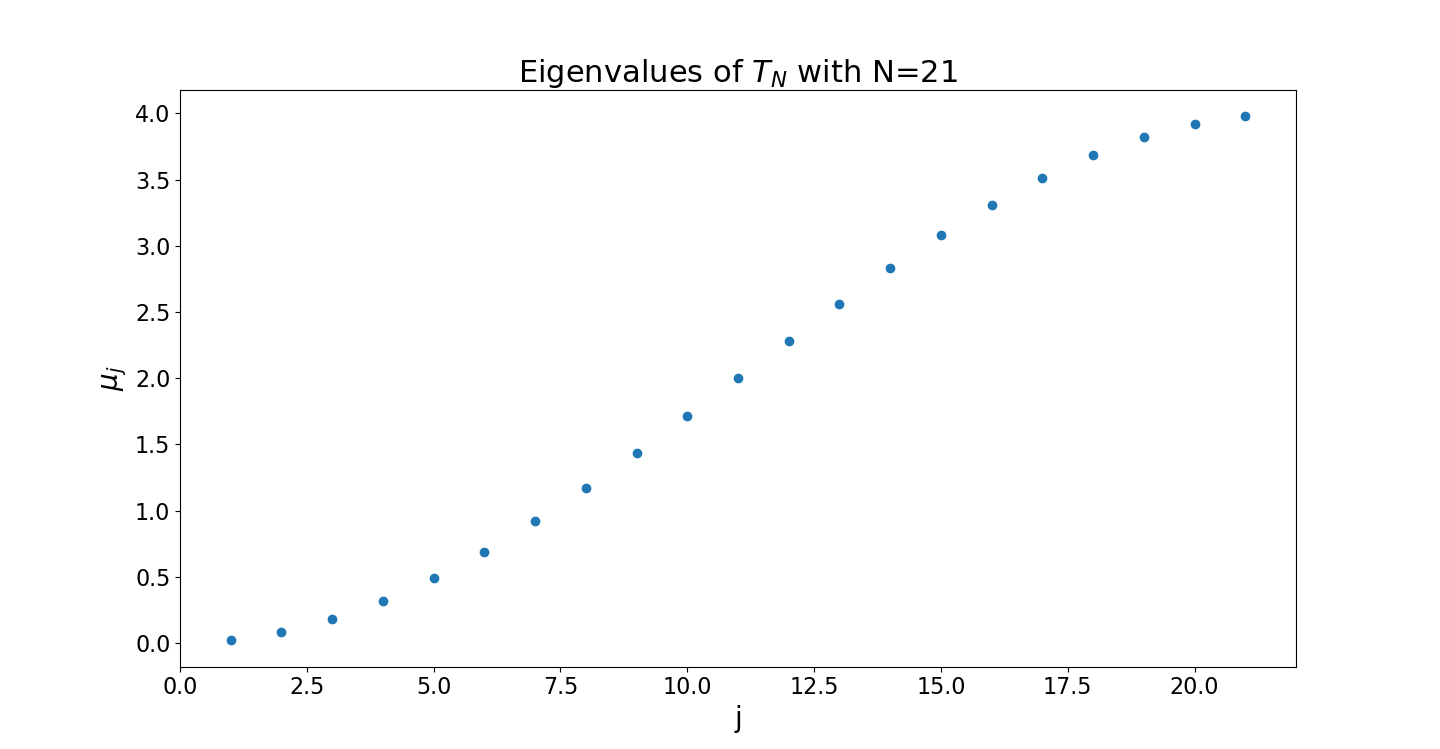
\includegraphics[scale=0.40]{Plot/Eigs_Tn_n=21.png}
	\caption{Eigenvalues of $T_{N}$, with $N=21$.}
	\label{Fig:Eigs_Tn}
\end{figure}

\begin{figure}[H]
%	\centering
	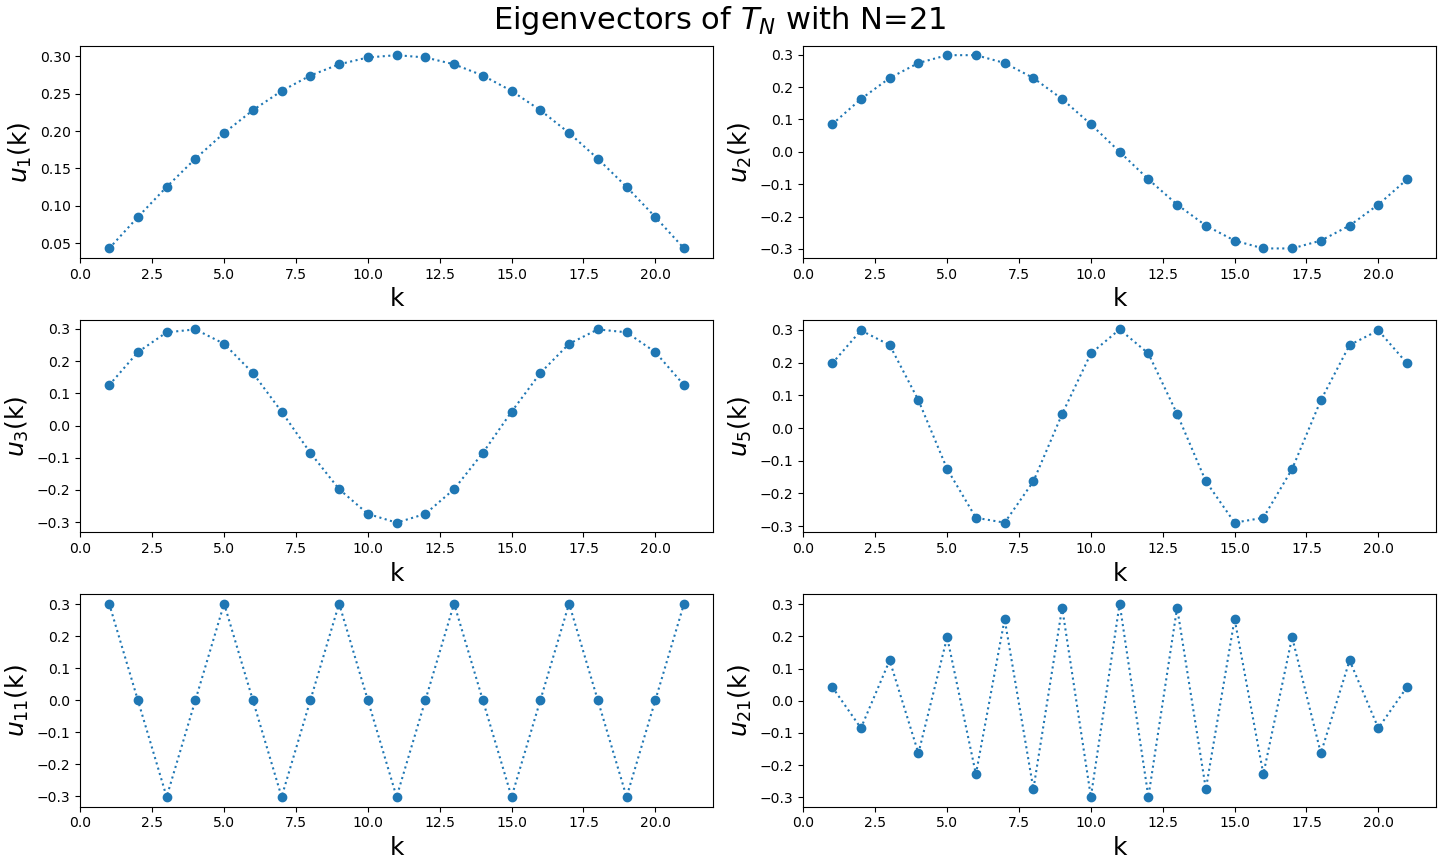
\includegraphics[scale=0.43]{Plot/Eigvect_Tn_n=21.png}
	\caption{Eigenvectors of $T_{N}$ for different values of $j$, with $j$ being the number that identifies the j-th eigenvector.}
	\label{Fig:Eigvect_Tn}
\end{figure}

\noindent \textbf{(6)} In the following we report the script implementing the inverse power method to find the smallest eigenvalue of $h^{-2}T_{N}$.

\begin{minted}[mathescape, linenos, breaklines]{python}
import numpy as np
import scipy

# Set initial parameters
N = 500
tol = 1e-8
initial_guess = np.random.random(N)
initial_guess = initial_guess/np.linalg.norm(initial_guess, ord=2)
count = 0
diff = 10 * tol

# Build T_N
T_N = scipy.sparse.diags([-1,2,-1],[-1,0,1],shape=(N,N)).toarray()

# Cholesky factorization of h^(-2)T_N
L, low = scipy.linalg.cho_factor(T_N)
L = (N+1) * L

vect_old = initial_guess

# Cycle until the difference in the 2-norm between two successive (approximated) eigenvectors is less than the chosen tolerance
while diff >= tol:
  # Compute and normalize the new vector by using the Choleski factorization of T_N
  vect_new = scipy.linalg.cho_solve((L, low),vect_old)
  vect_new = vect_new/np.linalg.norm(vect_new, ord=2)
  diff = np.linalg.norm(vect_new - vect_old, ord=2)
  count += 1
  vect_old = vect_new

# Compute the approximated eigenvalue
approx_eig = vect_new @ T_N @ vect_new * (N+1)**2

print(f'Iterations performed = {count}')
exact_eigval_T_N = 2 * (N+1)**2 * (1-np.cos(np.pi/(N+1)))
print(f'Absolute error eigenvalue) = {abs(approx_eig - exact_eigval_T_N)}')
index = np.array(range(1,N+1))
exact_eigvect = np.sqrt(2/(N+1)) * np.sin(index*np.pi/(N+1))
print(f'2-norm error eigenvector = {np.linalg.norm(vect_new - exact_eigvect, ord=2)}')
\end{minted}

\noindent The output of this code is the following:
\begin{minted}{text}
Iterations performed = 10
Absolute error eigenvalue = 1.531041959879076e-11
2-norm error eigenvector = 3.2570943203952573e-09
\end{minted}

\noindent As we can see, 10 iterations are required to obtain the chosen tolerance on the computed eigenvector. Finally, we report the plot of the computed eigenvector.
\begin{figure}[H]
	\centering
	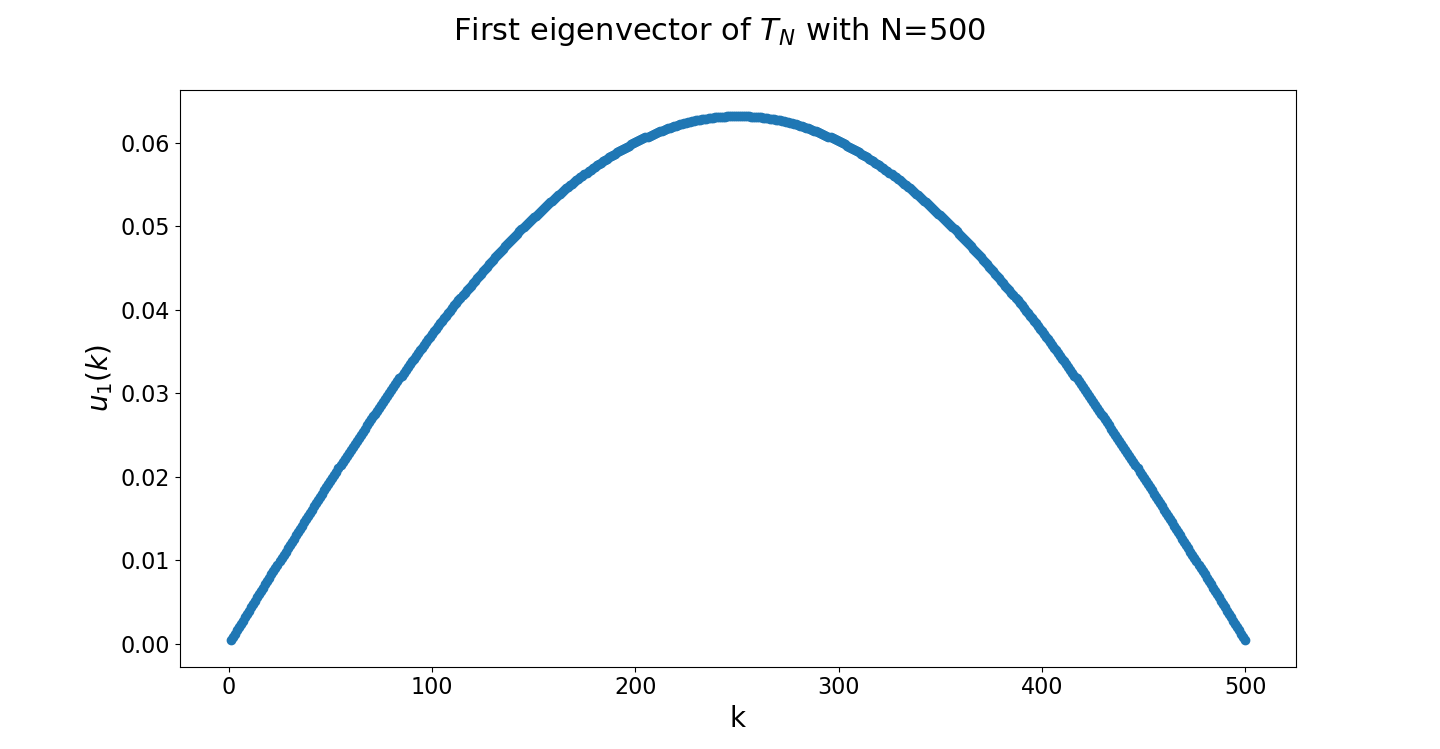
\includegraphics[scale=0.40]{Plot/First_eigvect_tn_n=500.png}
	\caption{First eigenvector of $T_{N}$, with $N=500$ computed by using the inverse power method.}
	\label{Fig:First_eigvect_Tn}
\end{figure}

\noindent \textbf{(7)} Below we report the script implementing the shift-and-invert method to find the fifth eigenvalue of $h^{-2}T_{N}$. In this case, it is not possible to use the Cholesky factorization since the matrix $h^{-2}T_{N} - 25\pi^2\mathbb{1}_{N}$ is not positive-definite.

\begin{minted}[mathescape, linenos, breaklines]{python}
import numpy as np
import scipy

# Set initial parameters
N = 500
lambda_5 = 25*np.pi**2
initial_guess = np.random.random(N)
initial_guess = initial_guess/np.linalg.norm(initial_guess, ord=2)
count = 0

# Build T_N
T_N = scipy.sparse.diags([-1,2,-1],[-1,0,1],shape=(N,N)).toarray()

tol = 1e-12 * np.linalg.norm((N+1)**2 * T_N, ord = np.inf)
diff = 10 * tol

# LU factorization of h^(-2)T_N
lu, piv = scipy.linalg.lu_factor(T_N*(N+1)**2 - lambda_5 * np.eye(N))

vect_old = initial_guess

# Cycle until the stopping criterion is satisfied - condition on the residual
while diff >= tol:
  # Compute and normalize the new vector by using the LU factorization to solve a linear system
  vect_new = scipy.linalg.lu_solve((lu, piv), vect_old)  
  vect_new = vect_new/np.linalg.norm(vect_new, ord=2)
  # Compute the approximated eigenvalue
  approx_eig = vect_new @ T_N @ vect_new * (N+1)**2
  diff = np.linalg.norm(( T_N * (N+1)**2 - approx_eig * np.eye(N) ) @ vect_new, ord=np.inf)
  count += 1
  vect_old = vect_new

print(f'Iterations performed = {count}')
exact_eigval_T_N = 2 * (N+1)**2 * (1-np.cos(5*np.pi/(N+1)))
print(f'Absolute error eigenvalue = {abs(approx_eig - exact_eigval_T_N)}')
index = np.array(range(1,N+1))
exact_eigvect = np.sqrt(2/(N+1)) * np.sin(index*np.pi*5/(N+1))
print(f'2-norm error eigenvector = {np.linalg.norm(vect_new - exact_eigvect, ord=2)}')
\end{minted}

\noindent The output of this code is the following:
\begin{minted}{text}
Iterations performed = 2
Absolute error eigenvalue = 1.0032863428932615e-11
2-norm error eigenvector = 5.021569614559994e-08
\end{minted}

\noindent In this case, 2 iterations are required to obtain an accurate approximation of the fifth eigenvector. Finally, we report the plot of the computed eigenvector.
\begin{figure}[H]
	\centering
	\includegraphics[scale=0.40]{Plot/Fifth_eigvect_tn_n=500.png}
	\caption{Fifth eigenvector of $T_{N}$, with $N=500$ computed by using the inverse shift-and-invert algorithm.}
	\label{Fig:Fifth_eigvect_Tn}
\end{figure}

\end{document}